\documentclass[11pt,a4paper]{article}

% ============================================================================
% PACKAGES
% ============================================================================
\usepackage[utf8]{inputenc}
\usepackage[T1]{fontenc}
\usepackage{amsmath,amssymb,amsthm}
\usepackage{mathtools}
\usepackage{algorithm}
\usepackage{algpseudocode}
\usepackage{graphicx}
\usepackage{booktabs}
\usepackage{multirow}
\usepackage{hyperref}
\usepackage{cleveref}
\usepackage{xcolor}
\usepackage{tikz}
\usetikzlibrary{shapes,arrows,positioning,fit,backgrounds,calc}
\usepackage[margin=1in]{geometry}
\usepackage{enumitem}
\usepackage{caption}
\usepackage{subcaption}

% ============================================================================
% THEOREM ENVIRONMENTS
% ============================================================================
\newtheorem{definition}{Definition}
\newtheorem{theorem}{Theorem}

% ============================================================================
% CUSTOM COMMANDS
% ============================================================================
\newcommand{\vect}[1]{\mathbf{#1}}
\newcommand{\mat}[1]{\mathbf{#1}}
\newcommand{\set}[1]{\mathcal{#1}}

% ============================================================================
% DOCUMENT
% ============================================================================
\begin{document}

Title - Methodology - Learning Automata for Adaptive Kelp Forest Monitoring 
PhD Thesis Research 
University of Victoria 
Date - Today

This chapter explains a method for adaptive monitoring of kelp forests. Satellite based environmental monitoring faces a basic problem - detection methods need feedback to improve but feedback arrives rarely and at unpredictable times. We offer a Learning Automata framework that keeps a pool of different detection methods and learns to choose among them according to the environmental setting. The framework has three linked parts - global policy learning, context aware adaptation plus sparse label handling. A main contribution is the dual layer non-stationarity model. This new extension of classical Learning Automata theory deals with shifting environmental conditions and irregular feedback timing at the same time. We test the approach with Leave-One-Site-Out evaluation along the coastal kelp forests of British Columbia.

\tableofcontents
\newpage


\section{The Monitoring Challenge}
\label{sec:challenge}

British Columbia hosts kelp forests that belong to the planet's most productive ecosystems. Dense stands of seaweed create shelter for multitudes of marine organisms, lock carbon into plant tissue and yield food plus materials that coastal First Nations have harvested for thousands of years. Ocean warming, acute marine heat events and expanding sea urchin grazing now subject those forests to stress they never experienced before. Tracking the condition but also extent of kelp over large areas is a basic requirement for any effective conservation plan but the work turns out to be unexpectedly hard.

Satellite remote sensing provides the wide area view that coastline scale monitoring demands. The Sentinel-2 sensor records an image of every part of British Columbia's 25 000 km shoreline once every five days and each pixel represents a square ten metres on a side. The obstacle is no longer the collection of pictures - the obstacle is the conversion of those pictures into trustworthy maps that show where kelp occurs. Three linked problems render this conversion intrinsically hard.

\subsection{Environmental Heterogeneity}

No universal detection algorithm exists - a technique tuned for clear, quiet summer seas collapses once it meets turbid winter water. Bull kelp that grows on wave beaten outer coasts shows a response unlike the same species in sheltered inland sites. A kelp bed that covers sand reflects light in distinct bands compared with a bed that roofs a rocky reef. River outflows, industrial discharge and nearby land add unique interference at each place.

A concrete example shows the problem - a deep learning model trains on images from the central coast of British Columbia. It memorizes the spectral pattern that kelp displays under those exact conditions - the clarity of the water, the kinds of seafloor and the usual atmospheric state. When the same model processes images from the northern coast, the water holds different substances, the depths vary and neighbouring objects change. Accuracy drops. The system memorized a single rule for kelp but kelp demands a separate rule for every setting.

\subsection{Sparse and Delayed Validation}

Field measurements that serve as reference truth cost a large amount of money and demand complex logistics. A survey team needs a boat, trained divers plus calm weather. The rate of such work stays far behind the speed at which Sentinel-2 acquires new scenes. An image that the satellite records today often waits weeks or months before a diver checks the site and many scenes never undergo any on site check.

A core conflict appears at this point - any detection system needs feedback so that its accuracy rises. But feedback reaches the team at uneven intervals and without warning. Classic machine learning practice expects a thick set of labels that arrive at the same time as the data - the usual step is to train on those labeled records and then release the model. When the same system moves into live service, it must keep learning, because only scattered validation signals reach it once it is already running.

\subsection{Non-Stationary Conditions}

The environment and the observation method each evolve through the year. Kelp forests follow a seasonal rhythm - they surge in spring, reach full cover in summer then decline in autumn. Water properties also shift with the season - winter delivers storms, murky water plus low solar elevation. A detection plan that works in August will fail in February.

Climate variability on long timescales causes regime shifts - el Niño events change ocean temperatures and affect kelp physiology. Marine heatwaves trigger large die offs. A detection method calibrated for normal conditions often fails when anomalies occur.

The way observations occur shifts over time - field validation adheres to seasonal rhythms - the majority of surveys take place during summer, when weather and access are optimal. Budget cycles, weather related hold-ups plus transport limits create differences between years. Because of those factors, the speed at which feedback reaches planners cannot be forecast.

\subsection{The Core Question}

Those challenges link to one another - environmental heterogeneity implies that distinct methods suit distinct settings. Sparse feedback implies that we are unable to train a fresh model for every setting. Non stationarity implies that, even if we trained such a model, the best method would continue to shift.

This leads to a concrete question - What happens if we abandon the search for one optimal model and instead keep a collection of varied detection methods then train a system to choose the most suitable one for each case? What if we discover which method performs best under specific conditions, infer this relationship from limited feedback and revise the selection as the environment shifts?

We set out this exact approach in the present chapter.


The central idea is to choose a model instead of teaching one.

The usual way to handle machine learning treats the choice of model as a single decision. A person trains multiple models, tests each on a validation set, keeps the one with the highest score and releases it into service. After that, the parameters stay constant - the environment is treated as unchanging.

We propose a fundamentally different approach - treat model selection as an ongoing learning problem. Instead of committing to a single detection method, we maintain a pool of diverse methods, each with distinct strengths and weaknesses plus learn to select among them based on environmental context.

\subsection{A Committee of Experts}

This approach works like a panel of specialists, each trained for a distinct set of conditions. One specialist identifies kelp best when the sea is calm and the water is clear. A second specialist performs reliably when the water carries a lot of suspended sediment. A third specialist maintains accuracy when the sun sits low above the horizon. After a fresh satellite image reaches the system, the software inspects the scene for water clarity, solar elevation, season and geographic position then it activates the specialist whose training matches those parameters.

Selection follows a probabilistic rule, not a fixed one - a probability distribution stays in place for every expert and it shows how much trust we assign to each. When the committee holds three experts, we might now judge that Expert A gives a correct result sixty percent of the time, Expert B thirty percent besides Expert C ten percent. After feedback appears - that is, after we receive a validated prediction - we revise those probabilities. When Expert B surpasses our expectation, its probability rises and the remaining probabilities drop.

As time passes, the probability distribution becomes stable - the system identifies which experts it should trust for each context. This identification proceeds without interruption while the system operates and it uses only scarce feedback. No full model retraining is necessary. Periodic validation alone suffices to refresh the selection preferences.

\subsection{Why Learning Automata?}

This task - choosing actions when outcomes are uncertain - is exactly what Learning Automata handle. Researchers in control theory created LA during the 1960s to let machines adapt their choices in settings where no model of the world exists. Each automaton keeps a list of probabilities, one for every action. It picks an action - sampling from this list, observes a numeric reward or penalty then revises the list so that the chosen action becomes more or less likely next time.

Linear approximations display a set of properties that fit our problem.

The agent accepts sparse feedback - it does not wait for a response after every step. When a reward signal arrives, the agent uses it to adjust its policy. If no signal arrives, the agent keeps the current policy and continues to act.

\item \textbf{Non-stationarity handling:} LA adapts when the environment changes. When the best action changes across time, the probability distribution adjusts and converges to the new optimum.

- Convergence guarantees - If the model matches reality, LA reach the best action with proof. This firm result sets them apart from improvised rules.

\textbf{Einfachheit:} Die Aktualisierungsvorschriften benötigen wenig Rechenaufwand. Es entfällt die Berechnung von Gradienten, es entfällt Backpropagation - es bleibt nur die Anpassung von Wahrscheinlichkeiten.

We place the formal account of LA in Appendix~\ref{app:la-theory}. At this point, a plain description is enough. LA give a clear rule that decides, from scarce feedback and while the situation shifts, which expert the system should trust.


Section - Framework Overview
Label - sec:overview

This section outlines the complete design of the adaptive monitoring framework. The system ingests satellite image tiles and generates maps that locate kelp. It refines its choices of which tiles to prioritize - learning from occasional, sparse validation feedback.

\subsection{System Architecture}

The framework includes three parts that work together - figure~\ref{fig:architecture} shows those parts.

\begin{figure}[h]
\centering
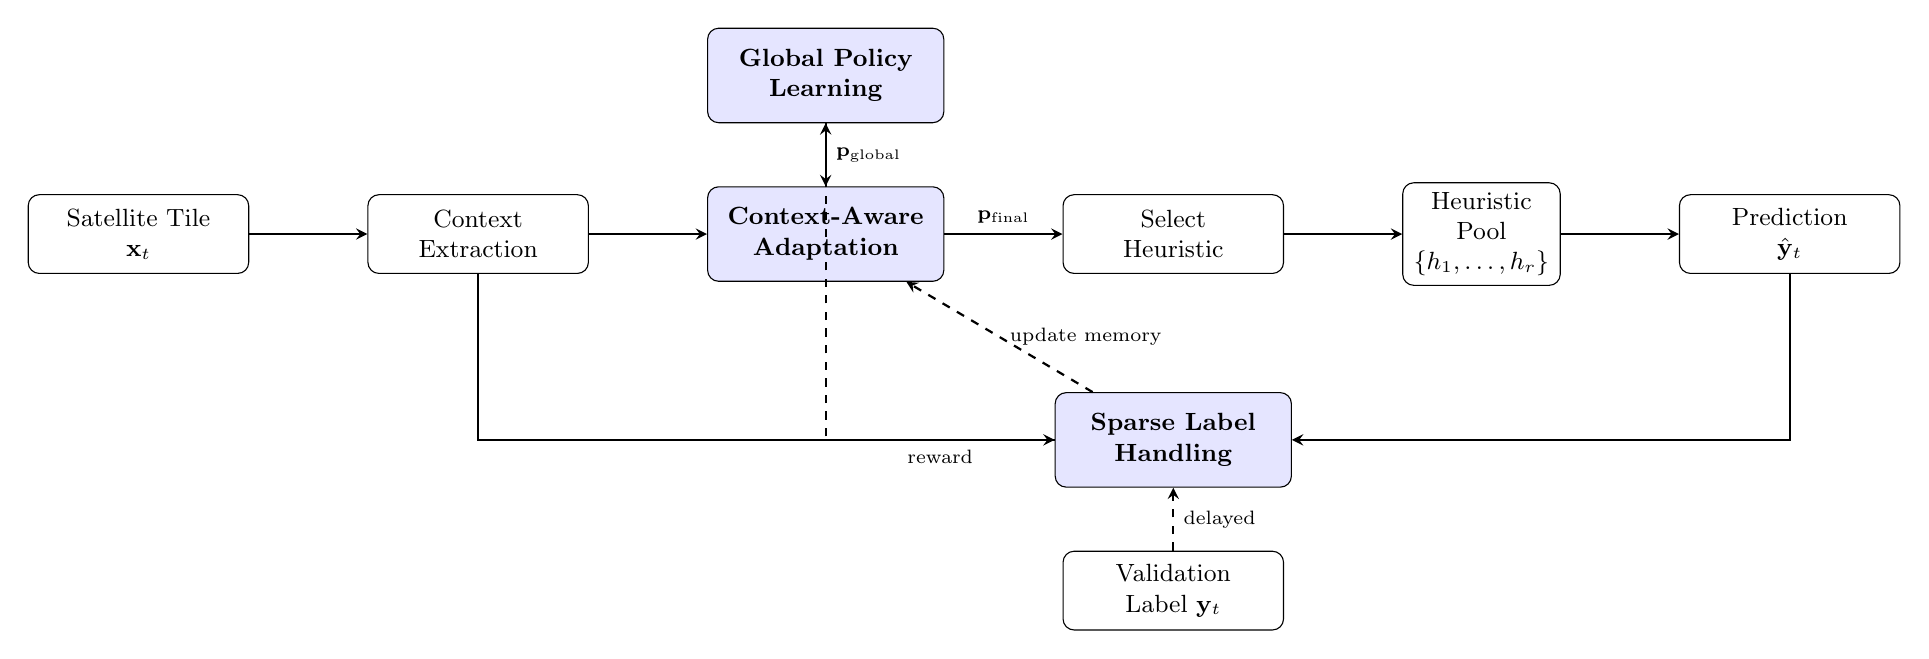
\begin{tikzpicture}[
    node distance=1.5cm,
    box/.style={rectangle, draw, rounded corners, minimum width=2.8cm, minimum height=1cm, align=center, font=\small},
    component/.style={rectangle, draw, rounded corners, fill=blue!10, minimum width=3cm, minimum height=1.2cm, align=center, font=\small\bfseries},
    arrow/.style={->, >=stealth, thick},
    dasharrow/.style={->, >=stealth, thick, dashed}
]
    % Input
    \node[box] (input) {Satellite Tile\\$\mathbf{x}_t$};

    % Context extraction
    \node[box, right=of input] (context) {Context\\Extraction};

    % Component 2
    \node[component, right=of context] (comp2) {Context-Aware\\Adaptation};

    % Component 1
    \node[component, above=0.8cm of comp2] (comp1) {Global Policy\\Learning};

    % Selection
    \node[box, right=of comp2] (select) {Select\\Heuristic};

    % Heuristic pool
    \node[box, right=of select, minimum width=2cm] (pool) {Heuristic\\Pool\\$\{h_1, \ldots, h_r\}$};

    % Prediction
    \node[box, right=of pool] (pred) {Prediction\\$\hat{\mathbf{y}}_t$};

    % Component 3
    \node[component, below=1.5cm of select] (comp3) {Sparse Label\\Handling};

    % Validation
    \node[box, below=0.8cm of comp3] (valid) {Validation\\Label $\mathbf{y}_t$};

    % Arrows
    \draw[arrow] (input) -- (context);
    \draw[arrow] (context) -- (comp2);
    \draw[arrow] (comp1) -- (comp2) node[midway, right, font=\scriptsize] {$\mathbf{p}_{\text{global}}$};
    \draw[arrow] (comp2) -- (select) node[midway, above, font=\scriptsize] {$\mathbf{p}_{\text{final}}$};
    \draw[arrow] (select) -- (pool);
    \draw[arrow] (pool) -- (pred);

    % To buffer
    \draw[arrow] (pred) |- (comp3);
    \draw[arrow] (context) |- (comp3);

    % From validation
    \draw[dasharrow] (valid) -- (comp3) node[midway, right, font=\scriptsize] {delayed};

    % Feedback loops
    \draw[dasharrow] (comp3) -| (comp1) node[near start, below, font=\scriptsize] {reward};
    \draw[dasharrow] (comp3) -- (comp2) node[midway, right, font=\scriptsize] {update memory};

\end{tikzpicture}
\caption{Framework architecture. Solid arrows show the inference path; dashed arrows show feedback paths that operate when validation labels arrive.}
\label{fig:architecture}
\end{figure}

The system keeps a probability list that covers every detection heuristic in the pool. 
This list records which heuristics achieved good results in the past. 
Once new feedback reaches the system, the list changes under Learning Automata rules.

The Context Aware Adaptation module examines the surroundings of every input tile. It stores a record of earlier encounters in a memory bank and adjusts the global preferences to match the present setting. When the system recognises the situation, it relies on the stored record. When the situation is new, it returns to the global preferences.

Sparse Label Handling stores forecasts until the true label appears. The label can arrive days, weeks or months after the forecast. Once the label is available, the system fetches the stored forecast, calculates the reward and then sends update signals to Component 1 and Component 2.

\subsection{The Inference Path}

When a fresh satellite tile reaches the system, the processing sequence begins in this way:

Extract context. 
The system retrieves environmental attributes from the tile - spectral statistics, texture values, the calendar day and the geographic coordinates. Those attributes combine into a context vector that records the prevailing state of the scene.

The system fuses worldwide and nearby preferences - it employs the context vector to search the memory bank for earlier situations that resemble the present one. When it finds such contexts and their recorded results stay uniform, it merges their preferences with the global policy. If the context has never appeared before, the system depends chiefly on the global policy.

A heuristic is chosen - drawing from a blended probability distribution. The choice is random - even heuristics that carry a low probability still appear from time to time, which keeps the search process open to new possibilities.

The chosen method examines the tile and returns a binary mask that labels each pixel as kelp or no kelp.

The system stores the forecast - the forecast, the context vector that belongs to it and the number of the chosen heuristic move into a buffer until the validator checks them.

\subsection{The Feedback Path}

The validation label arrives, sometimes weeks after we produced the original prediction. We process it in the following way:

The program fetches the buffered prediction. 
It uses the stored location and the exact timestamp to find the matching record inside the buffer.

Compute the reward - we assess the degree to which the prediction aligns with the ground truth label and we normally quantify this match with the Intersection-over-Union metric.

The reward signal changes the probability distribution across heuristics. When a heuristic performs well, its probability rises - when it performs poorly, its probability falls or it stays the same, according to the learning automaton scheme.

Update the memory bank - storing the context vector and the observed performance - this addition enriches later context aware adaptation.

The central point is that those feedback updates operate separately from inference. The system keeps generating predictions and does not pause until confirmation shows up. Once confirmation arrives, the system acquires new knowledge. But the acquisition happens out of step, occurs only now plus then and lags behind the moment of prediction.


% ============================================================================
\section{Component 1: Discovering Effective Methods}
\label{sec:component1}
% ============================================================================

The first component holds the system's global preferences for detection heuristics. It acts as the system's general view on which methods usually perform well, based on an average of all contexts it has experienced.

\subsection{The Probability Distribution}

The global policy is a probability distribution over $r$ heuristics:
\[
\mathbf{p} = [p_1, p_2, \ldots, p_r]
\]
where each $p_i$ represents the system's confidence in heuristic $h_i$. Initially, the distribution is uniform; the system has no prior preference:
\[
p_i(0) = \frac{1}{r} \quad \text{for all } i
\]

Feedback arrives step by step - each step shifts the probability assigned to every heuristic. A heuristic that returns high reward gains extra probability - a heuristic that returns low reward yields probability. After enough steps, almost the entire probability rests on the heuristics that deliver the highest reward.

\subsection{The Update Rule}

A reward is calculated once a forecast that relied on heuristic $h_i$ receives confirmation. This reward $R$ equals 0 when the detection fails entirely and equals 1 when the detection succeeds without error.

Probability adjustment relies on the chosen learning automata rule. The most basic rule, Linear Reward Inaction, changes the probability vector only after the environment returns a reward.

\begin{itemize}
\item When the reward lies above the threshold that marks acceptable performance, raise the probability $p_i$ and scale the remaining probabilities down so that their relative proportions stay intact. 
\item When the reward falls short of that threshold, leave every probability untouched. 
\end{itemize}

The system tolerates noise because it refrains from penalising a heuristic after one bad result. It withholds reward until the heuristic shows repeated good results. We list the exact update equations in Appendix~\ref{app:la-theory}.

We test six versions of three alternative algorithms - Linear Reward Penalty, Pursuit besides Variable Structure - because each balances learning speed against stability in a distinct way. The variants appear in Appendix~\ref{app:la-theory}. Through ablation studies we determine which variants detect kelp most effectively.

\subsection{Why This Works}

The global policy acts as the system's default preference - when no context specific data exists, it offers the best available estimate. It gains strength - combining experience from every context. If heuristic h3 succeeds in seventy percent of varied conditions, the system records a high p3.

Global settings treat every situation the same - a rule that works well in hot months often fails in cold months. The single policy smooths away such seasonal differences. A second module is necessary so that the system can adapt to each distinct context.


Component 2: Adapting to Context 
\label{sec:component2}

The second component allows the system to adjust its choice of heuristic according to the surrounding context. The logic is simple - when present conditions match earlier situations in which a specific heuristic performed well, the system gives preference to that heuristic.

\subsection{Context Features}

Each satellite tile holds data that describe the environmental situation present when the image was taken. We pull out a context vector $\mathbf{c}$ that encodes the following:

Spectral statistics - The mean and variance for every spectral band record the color of the water, its turbidity plus the state of the atmosphere. 
Spatial texture - Entropy and homogeneity values show how rough the surface is but also describe the wave pattern. 
Temporal context - The calendar day of the year records the seasonal cycle. 
Geographic location - Latitude and longitude record the properties of the region. 
Auxiliary data - Where it exists, bathymetry as well as substrate type are added.

This vector condenses the nature of the conditions that the system handles. If two tiles contain almost identical vectors, they probably need the same detection approach.

\subsection{The Memory Bank}

We keep a memory bank that stores past experiences. 
The bank has the form 
\[
\mathcal{M} = \{(\mathbf{c}_j, \mathbf{p}_j, R_j)\}
\] 
Each entry holds a context vector, the heuristic selection probabilities that were active under that context and the reward that followed. As time passes, the memory bank grows into a log that links each context to the choices that succeeded.

A fresh tile carries a context vector c - we look for the k contexts that lie closest to it in the stored collection. To scan a large memory bank quickly, we use FAISS, a software library that performs approximate nearest neighbor search at high speed.

\subsection{Local Preference Estimation}

The system fetches a set of neighbors - each neighbor shows which action succeeds under conditions that match the current state. We treat every neighbor as evidence. We weigh its preference score by its reward and by its cosine similarity to the present state. We add the weighted scores and divide by the sum of the weights. The result is a local probability distribution over actions.

Neighbors that resemble the current context and that received high rewards supply a larger portion of the local estimate. The outcome of this procedure is a distribution $\mathbf{p}_{\text{local}}$ that shows what succeeded under comparable conditions.

\subsection{Blending Global and Local}

The final selection probability blends global and local preferences:
\begin{equation}
\mathbf{p}_{\text{final}} = \alpha \cdot \mathbf{p}_{\text{global}} + (1 - \alpha) \cdot \mathbf{p}_{\text{local}}
\label{eq:blending}
\end{equation}

The blending coefficient $\alpha$ sets the balance. 
If $\alpha$ equals 1, the system follows only the global policy and discards local context. 
If $\alpha$ equals 0, the system relies only on local experience plus disregards global trends. 
For values between 0 and 1, the system combines information from both sources.

The system adjusts the weight $\alpha$ in response to the contents of the memory bank. If the bank stores numerous contexts that resemble one another and that lead to steady outcomes, the value of $\alpha$ drops - the model relies on local experience. If the stored contexts are new or their outcomes vary, the value of $\alpha$ rises - the model returns to global preferences.

\subsection{Why This Works}

Context-aware adaptation relies on patterns that exist within the problem. Environmental states do not occur at random - they form groups. When winter water in the Strait of Georgia is turbid, it resembles other winter turbid states in that same area. If a specific heuristic works under such states, it will probably work when they return.

The memory bank stores past solutions so the system can reuse them instead of learning a new model. No training links context features to heuristic success. The method recalls stored cases that match the present situation. It stays stable, allows clear inspection and needs no extra training phase.


RESULT_TOO_LONG

The third component addresses the practical situation in which validation labels appear only on occasion and at unpredictable intervals. The majority of predictions will never receive a label. When a label does arrive, it may show up days, weeks or even months after the original prediction. Despite this delay, the system must keep working and must not pause until feedback arrives. At the same time, it must incorporate the label once it appears.

\subsection{The Prediction Buffer}

Each forecast is stored in a buffer
\[
\mathcal{B} = \{(t_j, \mathbf{c}_j, i_j, \hat{\mathbf{y}}_j)\}
\] 
For every element, the buffer holds the exact time, the context vector, the index of the chosen heuristic and the predicted mask. A hash map permits rapid retrieval by place plus time.

A validation label reaches us for a specific place and day - we fetch the stored prediction that relates to that place plus day, calculate the reward and initiate updates for Component 1 and Component 2. After that step, we delete the item from the buffer.

\subsection{Buffer Management}

Forecasts do not stay valid forever - conditions in the environment shift - a forecast created six months earlier can lose value for present learning. The system enforces a strict upper limit on buffer age, for example six months. Any forecast that exceeds this limit is removed and receives no further revision.

This embodies our design philosophy - the system must learn from feedback that arrives while the situation is still current, not from feedback that arrives long after the event. A reward that reaches the system at once carries more information than a reward that reaches the system once the environment has already changed.

\subsection{Temporal Decay}

The system reduces a reward when validation occurs after the prediction. 
The effective reward equals the original reward multiplied by the decay factor raised to the power of the delay counted in days. 
The delay is the number of days between the moment of the prediction and the moment of the validation. 
The decay factor is a constant value below one. 
Feedback that arrives soon after the prediction keeps its full value. 
Feedback that arrives long after the prediction receives a smaller value.

This decay fulfils two objectives. 
It gives priority to recent data because the newest observations relate more closely to present circumstances. 
It monitors non stationarity - when the best heuristic shifts across time, the down weighting of earlier rewards lets the system adjust.

\subsection{Learning Without Waiting}

The central design rule is asynchronous learning - the inference path, which takes a tile as input and outputs a prediction, runs without pause plus does not wait for validation. The feedback path, which takes a label as input and outputs an update, runs whenever a label arrives. Those two paths operate independently.

This design reflects how environmental monitoring works in practice. Satellites collect images once every few days. Field teams perform validation when they have the resources and when weather plus logistics allow. The system does not pause prediction until validation data appear but it updates its models as soon as validation data arrive.


% ============================================================================
\section{Novel Element - Two Level Change Over Time}
\label{sec:dual-layer}
% ============================================================================

Classical Learning Automata theory studies systems that must pick actions in situations where the best choice shifts across time. This paper widens the theory so that it covers a further source of change - the moment at which information about the best action arrives also varies.

\subsection{Two Sources of Change}

Monitoring of kelp forests faces two separate forms of non stationarity that analysts need to address at the same time.

\begin{figure}[h]
\centering
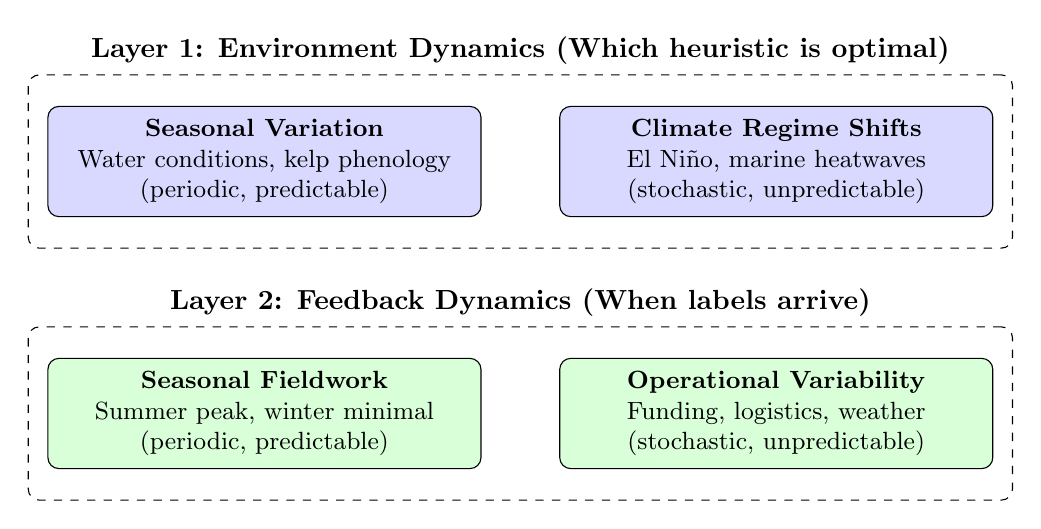
\begin{tikzpicture}[
    box/.style={rectangle, draw, rounded corners, minimum width=5.5cm, minimum height=1.4cm, align=center, font=\small},
    layer/.style={rectangle, draw, dashed, rounded corners, minimum width=12.5cm, minimum height=2.2cm}
]
    % Layer 1
    \node[box, fill=blue!15] (layer1-pse) at (-3, 2) {\textbf{Seasonal Variation}\\Water conditions, kelp phenology\\(periodic, predictable)};
    \node[box, fill=blue!15] (layer1-mse) at (3.5, 2) {\textbf{Climate Regime Shifts}\\El Ni\~{n}o, marine heatwaves\\(stochastic, unpredictable)};
    \node[layer, fit=(layer1-pse)(layer1-mse), label={[font=\bfseries]above:Layer 1: Environment Dynamics (Which heuristic is optimal)}] {};

    % Layer 2
    \node[box, fill=green!15] (layer2-pse) at (-3, -1.2) {\textbf{Seasonal Fieldwork}\\Summer peak, winter minimal\\(periodic, predictable)};
    \node[box, fill=green!15] (layer2-mse) at (3.5, -1.2) {\textbf{Operational Variability}\\Funding, logistics, weather\\(stochastic, unpredictable)};
    \node[layer, fit=(layer2-pse)(layer2-mse), label={[font=\bfseries]above:Layer 2: Feedback Dynamics (When labels arrive)}] {};
\end{tikzpicture}
\caption{Dual-layer non-stationarity model. Layer 1 governs which detection method is optimal. Layer 2 governs when validation feedback is available. Both layers combine periodic (seasonal) and stochastic (inter-annual) components.}
\label{fig:dual-layer}
\end{figure}

\subsubsection{Layer 1: Environment Dynamics}

This layer shows how the best detection rule shifts through time. Two distinct mechanisms cause the shift.

Kelp forests repeat the same sequence each year - during summer, the surface canopy reaches full size and sensors locate it without difficulty. Winter storms break off large sections of the canopy and suspended sediment clouds the water. An algorithm that locates kelp in clear summer water will probably miss plants in cloudy winter water. The most reliable rule for detection changes in a regular way that matches the seasons.

\item \textbf{Climate regime shifts (stochastic):} 
Year-to-year variation brings sudden, random changes - el Niño events raise or lower sea temperatures and disrupt kelp metabolism. Marine heatwaves create conditions that lack any earlier match. Each upheaval favours a different heuristic but the timing of the next shift remains unknown.

Classical LA theory labels the first type Periodic Switching Environment and the second type Markovian Switching Environment. Layer 1 merges both types.

\subsubsection{Layer 2: Feedback Dynamics}

The layer represents the moment when validation labels reach the system. It adds a new element to LA theory. Two mechanisms control when feedback appears:

Many validation surveys occur in summer, when weather and sea conditions allow boat based fieldwork. Winter validation is rare. The probability of receiving feedback follows a seasonal pattern.

\item \textbf{Operational variability (stochastic):} The amount of research money changes from year to year. Field teams are not always available at the same rate. Weather causes delays and equipment breaks - work stops without warning. In certain years, researchers collect many validation measurements - in other years, they collect few.
\end{itemize}

Layer 2 operates on its own and does not depend on Layer 1. 
A summer day can present ideal detection conditions within Layer 1 while Layer 2 still shows a high chance of feedback. 
A winter day can offer difficult detection conditions within Layer 1 while Layer 2 shows a low chance of feedback. 
The states of the two layers do not have to match.

\subsection{Why This Matters}

Classical LA theory centers on Layer 1 - the environment changes and the automaton must follow the shifting best action. This theory silently presumes that feedback appears at fixed intervals. In real systems, feedback arrives under its own timing rules.

The dual layer model reflects this situation. 
The system endures long stretches without feedback - during winter, multiple months often elapse before any validation arrives. The system must preserve steady behavior while it receives no updates.

\item \textbf{The system receives sudden feedback surges.} During summer, multiple surveys validate predictions within a short period. The system must absorb and process this feedback without delay.

The best action and the chance to receive feedback often move in opposite directions. When winter conditions arrive, some heuristics perform well but they yield sparse validation data. The system then acquires little knowledge about the exact situations that most demand adaptation.

When we model both layers in an explicit way, we analyse how learning evolves under conditions that reflect real world events. We create LA schemes that stay stable while droughts occur and that react quickly when bursts appear. We evaluate how robust the schemes remain when we alter the pattern of feedback.

\subsection{Scientific Contribution}

The dual layer non-stationarity model supplies three advances.

Novel theoretical extension - We extend the established theory of learning automata so that it treats feedback timing as its own random process in settings that change over time. This creates new analytical questions - How does learning performance decline when feedback arrives only rarely? Which learning automata schemes remain stable when the timing of feedback varies?

\item \textbf{Domain-appropriate modeling:} The formulation records actual attributes that belong to environmental monitoring. Seasonal patterns and operational variability exist as facts. When the model states them outright, the outcome gains realism.

The two layers allow separate configuration - researchers test the impact of Layer 1, which controls environment dynamics, while they freeze Layer 2 at a fixed setting. They then reverse the procedure, testing Layer 2 while Layer 1 remains unchanged. This separate control supports strict experimental study of how each source of non stationarity influences learning.


Section - Evaluation Strategy 
Label - sec:evaluation

We tested the framework on photographs of kelp forests taken along the coast of British Columbia. The test used Leave-One-Site-Out cross validation and followed a staged ablation protocol.

\subsection{Datasets}

\begin{table}[h]
\centering
\caption{Datasets used for evaluation}
\label{tab:datasets}
\begin{tabular}{lccp{5cm}}
\toprule
\textbf{Dataset} & \textbf{Images} & \textbf{Labels} & \textbf{Purpose} \\
\midrule
BC Sentinel-2 (Labeled) & 7 & Yes & Primary training and validation \\
BC Sentinel-2 (Multi-temporal) & $\sim$100 & No & Layer 1 testing, sparse simulation \\
Figshare Landsat & 432 & Yes & Cross-sensor transfer \\
\bottomrule
\end{tabular}
\end{table}

The main dataset holds Sentinel-2 images that cover seven coastal sites in British Columbia. Each image tile measures 512 by 512 pixels and each pixel represents a ground square of ten metres. Every tile stores twelve spectral and auxiliary bands. Analysts who specialise in coastal ecology have drawn precise kelp masks for each tile. Complete dataset details appear in Appendix~\ref{app:datasets}.

\subsection{Heuristic Pool}

The heuristic pool contains two groups of models. 

Ten site specific models exist - each model uses a UNet-MaxViT architecture. Each model was trained with the Leave-One-Site-Out protocol - every model encountered a distinct set of training conditions. 

One RGB model exists - this model was trained on all BC sites while it used only the visual spectral bands. This choice allows the model to transfer to Landsat imagery that carries the same bands.

\subsection{Leave-One-Site-Out Protocol}

Primary evaluation proceeds - leaving one site out at a time. The LA framework learns from six sites. It is tested on the single site that was left out. This sequence is repeated until every one of the seven sites has served as the test site. The outcomes from all runs are combined.

The protocol evaluates how well a system adapts to new geographic areas that it has not encountered before. This ability is essential for large scale deployment along coastlines.

\subsection{Staged Ablation}

A complete test of every design option would demand tens of thousands of separate trials. To keep the experimental plan feasible, we use a stepwise method:

Stage 1: LA variant selection - we compare six LA schemes (L$_{\text{R-I}}$, L$_{\text{R-P}}$, VSLA, Pursuit, Discretized Pursuit, SERI) with the full system. We identify the two or three schemes that achieve the highest performance.

Stage 2: Component ablation. 
We test each subset of parts - the global module alone - the global module joined with the context module - the global module joined with the sparse module; and the complete system. We run each subset together with the best LA variants.

Stage 3: Tolerance for sparse labels - we test how the system reacts when we lower the number of labels to 100 percent, 50 percent, 10 percent or 5 percent of the original total, while we keep the delay pattern that performed best in the earlier step.

We test whether the inclusion of bathymetry, substrate and other auxiliary layers changes the outcome.

Stage 5: Cross sensor transfer - we test the RGB-trained model on the Figshare Landsat dataset.

This step-by-step method cuts the number of required computer runs from more than 46 000 to about 500 but it keeps the study scientifically sound.

\subsection{Baselines}

We evaluate our approach - comparing it with three reference methods. We test against random selection, where each heuristic has an equal chance of being picked at every step. We use the single heuristic that yields the highest average score when applied alone across all tasks. We include an oracle that always selects the heuristic which achieves the best result for every individual tile - this sets an upper limit that assumes advance knowledge of the outcome.

\subsection{Metrics}

Primary detection metrics
\begin{itemize}[noitemsep]
\item \textbf{Intersection over Union (IoU):} The ratio of the area shared by the predicted kelp mask and the true kelp mask to the total area covered by either mask.
\item \textbf{F1-score:} The harmonic mean of precision plus recall.
\end{itemize}

Los-angeles-specific metrics
\begin{itemize}[noitemsep]
\item \textbf{Convergence speed:} Number of steps required until the system attains ninety percent of its ultimate performance level.
\item \textbf{Final entropy:} Degree to which the probability distribution concentrates once convergence occurs.
\end{itemize}

We present the formal definitions in Appendix~\ref{app:metrics}.


% ============================================================================
\section{Summary}
\label{sec:summary}
% ============================================================================

This chapter sets out a step-by-step method for watching kelp forests that change over time. The method solves basic problems that appear when people use satellites to study the environment.

The central idea views detection as a selection task instead of a training task. We keep a collection of varied methods and we learn to choose one of them according to the context, rather than build a single model that must operate in every situation.

The framework contains three parts.

Global policy learning observes the general success of heuristics through Learning Automata.

Context aware adaptation adjusts the choice of heuristic to the present state of the environment - retrieving stored cases.

Sparse label handling allows the system to learn even when validation signals arrive rarely or late.

The new contribution consists of a dual layer non-stationarity model. This model extends classical LA theory so that it covers two sources of change - first, environmental conditions that vary over time - second, feedback that arrives at irregular moments. The construction gives a theoretical basis for learning when an operational monitoring system must work under real world constraints.

The evaluation procedure applies Leave-One-Site-Out cross validation to every coastal kelp forest site in British Columbia. It removes components in a staged manner to discover which configurations perform well and to check how the system behaves when feedback data are scarce.

The next chapters show test outcomes that confirm every part and that prove the framework works for kelp forest monitoring that adapts.


% ============================================================================
% APPENDICES
% ============================================================================
\appendix

\section{Formal Statement of the Problem}
\label{app:formal}

\subsection{Input Space}

A satellite image tile that was captured at time t is represented by the symbol x_t. This tile is a three dimensional array of real numbers shaped as B rows, each of size H by W. The first dimension B equals the count of spectral bands. The second and third dimensions give the tile's height plus width in pixels. For a Sentinel-2 product, B is 12, both H besides W are 512 and every pixel covers a ground square ten metres on a side.

The context vector $\mathbf{c}_t \in \mathbb{R}^D$ encodes environmental conditions:
\begin{equation}
\mathbf{c}_t = \left[ \mathbf{c}^{\text{spectral}}_t, \mathbf{c}^{\text{spatial}}_t, \mathbf{c}^{\text{temporal}}_t, \mathbf{c}^{\text{environ}}_t, \mathbf{c}^{\text{geo}}_t \right]^\top
\end{equation}

\subsection{Heuristic Pool}

The heuristic pool $\mathcal{H} = \{h_1, \ldots, h_r\}$ contains $r$ detection methods, each mapping tiles to binary masks:
\begin{equation}
h_i : \mathbb{R}^{B \times H \times W} \rightarrow \{0, 1\}^{H \times W}
\end{equation}

\subsection{Reward Function}

The primary reward is Intersection over Union:
\begin{equation}
R(\hat{\mathbf{y}}, \mathbf{y}) = \text{IoU}(\hat{\mathbf{y}}, \mathbf{y}) = \frac{|\hat{\mathbf{y}} \cap \mathbf{y}|}{|\hat{\mathbf{y}} \cup \mathbf{y}|} = \frac{\text{TP}}{\text{TP} + \text{FP} + \text{FN}}
\end{equation}

\subsection{Policy Objective}

We learn a policy $\pi : (\mathbf{x}, \mathbf{c}) \rightarrow \Delta^{r-1}$ maximizing expected reward:
\begin{equation}
\pi^* = \arg\max_\pi \mathbb{E}_{(\mathbf{x}, \mathbf{c}, \mathbf{y}) \sim \mathcal{D}} \left[ \sum_{i=1}^{r} \pi(\mathbf{x}, \mathbf{c})_i \cdot R(h_i(\mathbf{x}), \mathbf{y}) \right]
\end{equation}


\section{Automata Theory for Learning}
\label{app:la-theory}

\subsection{Basic Formulation}

\begin{definition}[Learning Automaton] 
A Learning Automaton is a four part object written as $\langle \mathcal{A}, \mathcal{R}, \mathbf{p}, T \rangle$ where
\begin{itemize}[noitemsep] 
\item $\mathcal{A} = \{\alpha_1, \ldots, \alpha_r\}$ is the set that lists every action the automaton is allowed to choose; 
\item $\mathcal{R} = \{0, 1\}$ is the set that contains the two possible responses from the environment: 0 stands for reward and 1 stands for penalty; 
\item $\mathbf{p}(n) = [p_1(n), \ldots, p_r(n)]^\top$ is the column vector that stores, for step $n$, the probability of selecting each separate action; 
\item $T$ is the fixed rule that revises every probability once the automaton receives a response. 
\end{itemize} 
\end{definition}

Each setting contains a set of penalty probabilities $\{c_1, \ldots, c_r\}$. For every element $c_i$, the value equals the conditional probability that the random variable $\beta$ takes the value 0 given that the random variable $\alpha$ equals the specific value $\alpha_i$.

RESULT_TOO_LONG

Update on reward only:
\begin{align}
\text{If } \beta(n) = 1: \quad & p_i(n+1) = p_i(n) + \alpha(1 - p_i(n)) \quad \text{(selected action)} \\
& p_j(n+1) = p_j(n)(1 - \alpha) \quad j \neq i \\
\text{If } \beta(n) = 0: \quad & p_i(n+1) = p_i(n) \quad \forall i
\end{align}

Theorem (L$_{\text{R-I}}$ Convergence) 
If the penalty probabilities differ and form a strict ascending sequence $c_1 < c_2 < \cdots < c_r$ then the L$_{\text{R-I}}$ scheme reaches the best action with probability one.

RESULT_TOO_LONG

Update on both reward and penalty:
\begin{align}
\text{If } \beta(n) = 1: \quad & p_i(n+1) = p_i(n) + \alpha(1 - p_i(n)) \\
& p_j(n+1) = p_j(n)(1 - \alpha) \quad j \neq i \\
\text{If } \beta(n) = 0: \quad & p_i(n+1) = p_i(n)(1 - \beta) \\
& p_j(n+1) = p_j(n) + \frac{\beta}{r-1}(1 - p_j(n)) \quad j \neq i
\end{align}

\subsection{Pursuit Automata}

We maintain reward estimates $\hat{d}_i(n)$ and pursue the current best:
\begin{align}
\hat{d}_i(n) &= \frac{\text{Total rewards for } \alpha_i}{\text{Total selections of } \alpha_i} \\
m(n) &= \arg\max_i \hat{d}_i(n) \\
p_{m(n)}(n+1) &= p_{m(n)}(n) + \alpha(1 - p_{m(n)}(n))
\end{align}

\subsection{Variable Structure LA (VSLA)}

Adaptive learning rate based on entropy:
\begin{align}
H(\mathbf{p}) &= -\sum_{i=1}^{r} p_i \log_2 p_i \\
\alpha(n) &= \alpha_{\min} + (\alpha_{\max} - \alpha_{\min}) \cdot \frac{H(\mathbf{p}(n))}{\log_2 r}
\end{align}

RESULT_TOO_LONG

Bayesian estimation starts from a Beta posterior for every parameter vector entry. 
Each posterior density has the form p(θ_i | data) ∝ Beta(α_i, β_i). 
The algorithm revises each pair (α_i, β_i) in the same way that pursuit methods revise action probabilities. 
The procedure needs minimal time to reach an ε-optimal policy.


\section{Algorithm Pseudocode}
\label{app:algorithms}

\begin{algorithm}[H]
\caption{Framework Inference}
\begin{algorithmic}[1]
\Require Tile $\mathbf{x}$, global policy $\mathbf{p}_{\text{global}}$, memory bank $\mathcal{M}$
\State $\mathbf{c} \gets \text{ExtractContext}(\mathbf{x})$
\State $\mathcal{N}_k \gets \text{kNN}(\mathbf{c}, \mathcal{M}, k)$
\State $\mathbf{p}_{\text{local}} \gets \text{WeightedAverage}(\mathcal{N}_k)$
\State $\alpha \gets \text{ComputeBlendingCoef}(\mathcal{N}_k)$
\State $\mathbf{p}_{\text{final}} \gets \alpha \cdot \mathbf{p}_{\text{global}} + (1-\alpha) \cdot \mathbf{p}_{\text{local}}$
\State $i \sim \text{Categorical}(\mathbf{p}_{\text{final}})$
\State $\hat{\mathbf{y}} \gets h_i(\mathbf{x})$
\State $\mathcal{B} \gets \mathcal{B} \cup \{(t, \mathbf{c}, i, \hat{\mathbf{y}})\}$ \Comment{Buffer prediction}
\State \Return $\hat{\mathbf{y}}$
\end{algorithmic}
\end{algorithm}

\begin{algorithm}[H]
\caption{Label Arrival Processing}
\begin{algorithmic}[1]
\Require Validation label $\mathbf{y}$ for location $\ell$, time $t$
\State $(t_j, \mathbf{c}_j, i_j, \hat{\mathbf{y}}_j) \gets \mathcal{B}[\text{lookup}(\ell, t)]$
\State $\delta \gets t_{\text{current}} - t_j$ \Comment{Delay}
\If{$\delta > T_{\max}$}
    \State Remove from buffer; \Return \Comment{Too old}
\EndIf
\State $R \gets \text{IoU}(\hat{\mathbf{y}}_j, \mathbf{y}) \cdot \gamma^\delta$ \Comment{Reward with decay}
\State $\mathbf{p}_{\text{global}} \gets \text{LAUpdate}(\mathbf{p}_{\text{global}}, i_j, R)$ \Comment{Update Component 1}
\State $\mathcal{M} \gets \mathcal{M} \cup \{(\mathbf{c}_j, \mathbf{p}_{\text{final}}, R)\}$ \Comment{Update Component 2}
\State Remove entry from $\mathcal{B}$
\end{algorithmic}
\end{algorithm}


\section{Dataset Details}
\label{app:datasets}

\subsection{BC Sentinel-2 Dataset}

\begin{table}[h]
\centering
\caption{BC Sentinel-2 sites}
\begin{tabular}{llllc}
\toprule
\textbf{Site} & \textbf{UTM} & \textbf{Date} & \textbf{Season} & \textbf{Tiles} \\
\midrule
T09UXQ & 9U & July 27, 2021 & Summer & $\sim$40 \\
T09UYQ & 9U & August 6, 2022 & Summer & $\sim$45 \\
T10UCU & 10U & August 6, 2022 & Summer & $\sim$50 \\
T09UXS & 9U & August 4, 2023 & Summer & $\sim$35 \\
T10UCA & 10U & August 16, 2023 & Summer & $\sim$40 \\
T09UWT & 9U & August 19, 2023 & Summer & $\sim$45 \\
T09UUU & 9U & September 2, 2023 & Summer & $\sim$42 \\
\midrule
\multicolumn{4}{l}{\textbf{Total}} & $\sim$300 \\
\bottomrule
\end{tabular}
\end{table}

\subsection{Band Specification}

\begin{table}[h]
\centering
\caption{12-band tile structure}
\begin{tabular}{cll}
\toprule
\textbf{Band} & \textbf{Source} & \textbf{Resolution} \\
\midrule
1--4 & B2, B3, B4, B8 & 10m (native) \\
5--10 & B5, B6, B7, B8A, B11, B12 & 10m (resampled from 20m) \\
11 & Substrate classification & 10m (resampled) \\
12 & Bathymetry & 10m (resampled) \\
\bottomrule
\end{tabular}
\end{table}


\section{Metrics Definitions}
\label{app:metrics}

\subsection{Detection Metrics}

\begin{align}
\text{IoU} &= \frac{\text{TP}}{\text{TP} + \text{FP} + \text{FN}} \\
\text{Precision} &= \frac{\text{TP}}{\text{TP} + \text{FP}} \\
\text{Recall} &= \frac{\text{TP}}{\text{TP} + \text{FN}} \\
\text{F1} &= 2 \cdot \frac{\text{Precision} \cdot \text{Recall}}{\text{Precision} + \text{Recall}}
\end{align}

\subsection{LA Metrics}

\begin{align}
\text{Entropy} &= H(\mathbf{p}) = -\sum_{i=1}^{r} p_i \log_2 p_i \\
\text{Convergence} &= \min\{n : \text{IoU}(n) \geq 0.9 \cdot \text{IoU}_{\text{final}}\}
\end{align}


The bibliography section starts here. 
The document selects the style named plain for the list of references. 
The list itself begins and is set to hold up to ninety nine entries.

K. S. Narendra besides K. S - thathachar wrote the book Learning Automata - An Introduction, which was published by Prentice Hall in 1989.

M. A. L. Thathachar besides P. S - sastry present a survey of the types of learning automata. The article appears in IEEE Transactions on Systems, Man or Cybernetics, Part B, volume 32, number 6, on pages 711 - 722, dated 2002.

S - b., Dupont, C., Boyer, L., Juanes, F. and Costa, M. employed passive remote sensing to chart bull kelp. The report appears in Global Ecology besides Conservation, volume 22, article identifier e00948, year 2020.

S. Starko and coworkers report that kelp forests along the British Columbia coast contain communities with pronounced heterogeneity. Their findings appear in the Journal of Phycology for the year 2024.

A. Mora Soto and co authors examine the difficulties that appear when researchers attempt to locate kelp forests across the entire planet by means of satellite images.

\end{thebibliography}

\end{document}
